%!TEX root = ..\main.tex
\section{Langevin Dynamics}
\label{sec:langevin_dynamics}

\subsection{Langevin equations}
\label{subsec:langevin_equations}
To study dynamics of system described in section \ref{sec:model} (again, in 1D tube), we apply the Langevin dynamics approach which follows the Langevin equation of (translational) motion
\begin{equation}
\label{eq:langevin_theory_1}
	\dot{r} = v
\end{equation}
\begin{equation}
\label{eq:langevin_theory_2}
	m \dot{v} = f(r, t) - \alpha v + \beta(t)
\end{equation}
where $\alpha$ --- is damping coefficient related with a drag force induced by a medium, and $f(r, t)$ is a force acting on a particle. $\beta$ is a stochastic force, and in order to satisfy dissipation-fluctuation theorem, it is assumed to be Gausian-distributed, and have statistical properties
\begin{equation}
\langle\beta(t)\rangle = 0,
\end{equation}
\begin{equation}
\langle\beta(t)\beta(t')\rangle = 2 \alpha k_B T\delta(t - t')
\end{equation}
where $k_B$ is the Boltzmann constant, $T$ is thermostat temperature and $\delta$ is the Dirac delta function.

For the rotational motion the form of equations remains unchanged, but one have to do a direct substitution of 
\begin{equation}
\label{eq:rotation_translation_substitution}
	\begin{aligned}[c]
		\phi &\rightarrow r        \\
		\omega &\rightarrow v 
	\end{aligned}
	\qquad
	\qquad
	\begin{aligned}[c]
		I &\rightarrow m        \\
		\tau(r, t) &\rightarrow f(r, t)
	\end{aligned}
\end{equation}
where $\phi$ is particle orientation angles, $\omega$ is angular velocity, $I$ is inertia and $\tau$ is torque exerted on a particle.

The damping coefficients $\alpha$ for translation ($\alpha_t$) and rotation ($\alpha_r$) are different, and can be defined in following way.

First to simplify the particle-solution interaction description we need to define damping time $\tau$, which determines how rapidly temperature is relaxed, and for translational motion it is given by
\begin{equation}
\label{eq:Translation_damping_time}
	\tau_{t} = \frac{m}{6 \pi \eta R}
\end{equation}
where $m$ is particle mass, $\eta$ is viscosity and $R$ is particle radius. For rotation $\tau_{t} / \tau_{r} = 10/3$, which can be \textcolor{red}{obtained from}

And than the $\alpha_t$ and $\alpha_r$ are defined
\begin{equation}
	\begin{aligned}
		\alpha_t = \frac{m}{\tau_t}
	\end{aligned}
	\qquad
	\qquad
	\begin{aligned}
		\alpha_r = \frac{I}{\tau_r}
	\end{aligned}
\end{equation}
where $m$ is particle mass, $I$ is inertia, $\tau_{t,r}$ is damping time

\subsection{Statistical properties}
For non-interacting spheres which are able to move and rotate freely in three dimensions and are immersed in a (fluid) medium, the relation between rotational and translational diffusion coefficient can be obtained.
The former is given by the Stokes-Einstein relation
\begin{equation}
	D_t = \frac{k_B T}{6 \pi \eta R}
\end{equation}
and the latter is given by Stokes-Einstein-Debye relation
\begin{equation}
	D_r = \frac{k_B T}{8 \pi \eta R^3}
\end{equation}
where $T$ is temperature, $\eta$ the viscosity of the fluid medium and $k_B$ the Boltzmann constant. The relation between $D_t$ and $D_r$ is given by
\begin{equation}
	\frac{D_r}{D_t} = \frac{3}{4 R^2}
\end{equation}

For sufficiently long integration times, we can find that
\begin{equation}
\label{eq:translation_diffsion_vs_displacement}
	D_t = \lim_{\Delta t \to \infty} \frac{1}{6 \Delta t} \langle r^2(\Delta t)\rangle
\end{equation}
where $\langle r^2(\Delta t)\rangle$ is translational mean square displacement of particle
\begin{equation}
	\langle r^2(\Delta t)\rangle
	 = \frac{1}{N} \sum_{i=1}^{N} |\vec{r}_i(t + \Delta t) - \vec{r}_i(t)|^2
\end{equation}

Analogously can be defined relation between rotational diffusion coefficient $D_r$ and rotational mean square displacement $\langle \phi^2 \rangle$ (RMSD)

\begin{equation}
\label{eq:rotational_diffsion_vs_displacement}
	D_t = \lim_{\Delta t \to \infty} \frac{1}{6 \Delta t} \langle \phi^2(\Delta t)\rangle
\end{equation}

Any rotation can be represented in a axis-angle way, so, we can define rotational displacement (RD) following \textcolor{red}{Kraft et al}
\begin{equation}
\label{eq:full_rotational_displacement}
	\Delta \vec{u}(t + \Delta t) 
		= \frac{1}{2} \sum_{i = 1}^{3} \Delta \vec{u}_i(t + \Delta t)
\end{equation}
where $\Delta \vec{u}_i(t + \Delta t)$ is RD of each vector in a set of orthogonal vectors. We can use e.g. ones which define reference frame connected with particle.

The direction of RD for any $\vec{u}_i$ is given by
\begin{equation}
\label{eq:rot_displ_i_direction}
	\Delta \hat{u}_i(t + \Delta t)
		= [\hat{u}_i(t) \times \hat{u}_i(t + \Delta t)]
\end{equation}
and the length is given by
\begin{equation}
\label{eq:rot_displ_i_magnitude}
	|\Delta \vec{u}_i(t + \Delta	 t)|
		= \cos^{-1}(\hat{u}_i(t) \cdot \hat{u}_i(t + \Delta t))
\end{equation}
i.e. $\Delta \vec{u}_i$ is the vector with magnitude of the angle between $\vec{u}_i(t)$ and $\vec{u}_i(t + \Delta t)$, and the direction perpendicular to the plane of rotation (i.e. the plane given by $u_i$ and $u_i(+dt)$).

The definition \eqref{eq:full_rotational_displacement} is bonded, and should be treated with care in case if particle can rotate on more than $2\pi$ radians within one time step. In that case $\Delta \vec{u}$ should be multiplied by $2 \pi$.

Using the definition \eqref{eq:full_rotational_displacement}, the RMSD can be obtained
\begin{equation}
\label{eq:rotational_mean_square_displacement}
	\langle \phi^2 (\Delta t)\rangle
		= \frac{1}{N} \sum_{i=1}^{N} 
			\left|
				\int_{t}^{t+\Delta(t)}
					\Delta \vec{u}(t + \Delta t) 
					- \Delta \vec{u}(t)
				dt
			\right|^2
\end{equation}

\textcolor{red}{By the way, I'm using $\Delta u$ instead of $\phi^{n+1} - \phi^{n}$, I believe I can use the $\omega" dt$ instead, since the values are the same, but which will be bore in lines with translation?}

\begin{figure}[h]
	\centering
	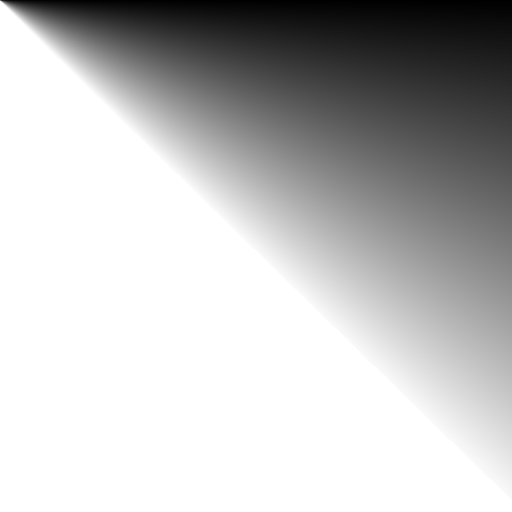
\includegraphics[width=0.5\textwidth, height=5cm]{Images/dummy.png}
	\caption{Molecular displacement as function of time}
	\label{fig:displacement_vs_time}
\end{figure}

\subsection{Integration method}
\label{subsec:integration_method}

The integration scheme for translational equations of motion is as follows

\begin{equation}
\label{eq:tr_coordinate_change}
	r^{n+1} = r^n + dt \left(
	 b_{t} v^n
	 + \frac{b_{t} dt}{2m}f^n
	 + \frac{b_{t}}{2m}\beta_{t}^{n+1}
	\right)
\end{equation}
\begin{equation}
\label{eq:tr_velocity_change}
	v^{n+1} = v^n 
	 + \frac{dt}{2m}\left(f^n + f^{n+1}\right)
	 - \frac{\alpha_{t}}{m}\left(r^{n+1} - r^n\right)
	 + \frac{1}{m}\beta_{t}^{n+1}
\end{equation}

where $b$ accounts for the drag exerted on a particle by surrounding medium,
\begin{equation}
\label{eq:drag_coefficient}
	b = \frac{1}{1 + \frac{\alpha dt}{2 m}}
\end{equation}

The same integration scheme can be used for rotation, with substitution defined in the eq. (\ref{eq:rotation_translation_substitution})
	
\begin{equation}
\label{eq:rot_angle_change}
	\phi^{n+1} = \phi^n + dt \left(
	  b_{r} \omega^n
	  + \frac{b_{r} dt}{2I}\tau^n
	  + \frac{b_{r} }{2I}\beta_{r}^{n+1}
	 \right)
\end{equation}
\begin{equation}
\label{eq:rot_ang_velocity_change}
	\omega^{n+1} = \omega^n
	+ \frac{dt}{2m}\left(\tau^n + \tau^{n+1}\right)
	- \frac{\alpha_{r}}{I}\left(\phi^{n+1} - \phi^n\right)
	+ \frac{1}{I}\beta_{r}^{n+1}
\end{equation}

When $\alpha = 0$, the above equations reduces to the standard velocity-Verlet scheme. The damping is represented by integration (under assumption that damping coefficient is constant) over real path travelled by particle within time step.

If using integration scheme defined in eq. (\ref{eq:rot_angle_change}), effective angular velocity of a particle within every time step is
\begin{equation}
\label{eq:effective_angular_velocity}
	\tilde{\omega}^n = b_{r} \omega^n
	+ \frac{b_{r} dt}{2I}\tau^n
	+ \frac{b_{r} }{2I}\beta_{r}^{n+1}
\end{equation}

By the definition, angular velocity $\omega$ is directed parallel to the axis around which body is rotated on the angle $|\omega|dt$ per time $dt$. Therefore, if particle orientation is defined by quaternion $q$, then
\begin{equation}
q^{n+1} = \tilde{q} q^{n}
\end{equation}
where $q^n$ and $q^{n+1}$ is the quaternion representation of orientation on time step $n$ and $n+1$ respectfully, and $\tilde{q} q^{n}$ is quaternion multiplication. \textcolor{red}{quaternions defined in appendix}. $\tilde{q}$ is the quaternion representation of rotation around $\tilde{\omega}$ on the angle $|\tilde{\omega}|$.

\subsection{Interactions}

For the MD simulations we used following equations:

\textcolor{red}{The energy and the field have same letters, what is standard practice to name field and energy?}
\begin{equation}
\label{eq:dipole_field}
	E_d = \frac{\mu}{r^3}
		\left(3 (\hat{\mu} \cdot \hat{r}) \hat{r} - \hat{\mu} \right)
\end{equation}
where $\mu$ is dipole moment of a particle producing field, and $r$ is distance to the point of measurement.

The dipole-dipole interaction potential \eqref{eq:dipole_dipole_interaction} can be expressed
\begin{equation}
\label{eq:dipole_energy_from_potential}
	E^{dip}_{12} = -(\mu_1 \cdot E_{d_2})
\end{equation}

Full force acting on a particle is
\begin{equation}
\label{eq:full_force}
	\vec{F}
		= \frac{\delta E_{12}}{\delta \vec{r}}
		= \hat{r} \frac{exp(-k r)}{r^4}(3 D exp(k r) - A r^2 (k r +1)
\end{equation}
where $D = 3 \cos \theta_1 \cos \theta_2 - (\hat{m}_1 \cdot \hat{m}_2)$ stands for orientational part of dipole-dipole potential. $\vec{r}$ is distance from other particle to one on which the force applies. The other parameters are the same as in eq. \eqref{eq:full_particle_particle_interraction}

The torque on a particle arises only due to dipole-dipole interaction. Therefore it is calculated as
\begin{equation}
\label{eq:dipole_torque}
	\tau  = \mu[\hat{\mu} \times E_d ]
\end{equation}
where $\vec{\mu}$ is dipole moment of particle on which torque acts, and $E_d$ is dipole field produced by acting particle.
